This paper introduces \texttt{yaw}, a language for algebraic quantum
programming. Before we dive into the details, it will be helpful to
recall what ``algebraic quantum programming'' means.\sidenote{For a
considerably lengthier version, we refer readers to the prequel paper, ``The Structure and Interpretation of
Quantum Programs I: Foundations'' (2025).}
Usually, quantum programming occurs at the level of a (typically
finite-dimensional) Hilbert space $\mathcal{H}$,
with basic objects the states $|\psi\rangle \in \mathcal{H}$. We
manipulate these using linear operators on the Hilbert space $A \in
\mathcal{B}(\mathcal{H})$; these are built out of primitive,
physically simple(r) operations $\mathcal{G} \subseteq \mathcal{B}(\mathcal{H})$ called ``gates'', and the whole
workflow of preparing a state $|\psi\rangle$, building an operation $A$ from simpler
gates, and extracting outputs from $A|\psi\rangle$,
is called a \emph{quantum circuit}.
The canonical example is to initialize $|\psi\rangle = |0^n\rangle$ in the Hilbert space of $n$ qubits,
$\mathcal{H} = \mathcal{H}_2^{\otimes n}$, generate
$\mathcal{B}(\mathcal{H})$ from a two-qubit universal gate set like
$\mathcal{G}=\{H_i, S_i, T_i, \text{CNOT}_{ij}\}$ where $i$ and $j$
indicate which qubits are acted on, and finally measure in the $Z$
basis.% \marginnote{This is of course something of a caricature, but it
  % is a common caricature.}

This is a fairly reasonable physical picture of what goes on inside
a quantum computer, provided we ignore the physical errors induced by
interactions with the environment.
But (even ignoring errors) certain limitations of the
circuit paradigm become apparent. The focus on compilation of
operators from gate sets makes the typical presentation of an
algorithm dense, obscure, and low-level. Here is Grover search for instance:

\begin{figure}[h]
  \centering
  \vspace{-10pt}
  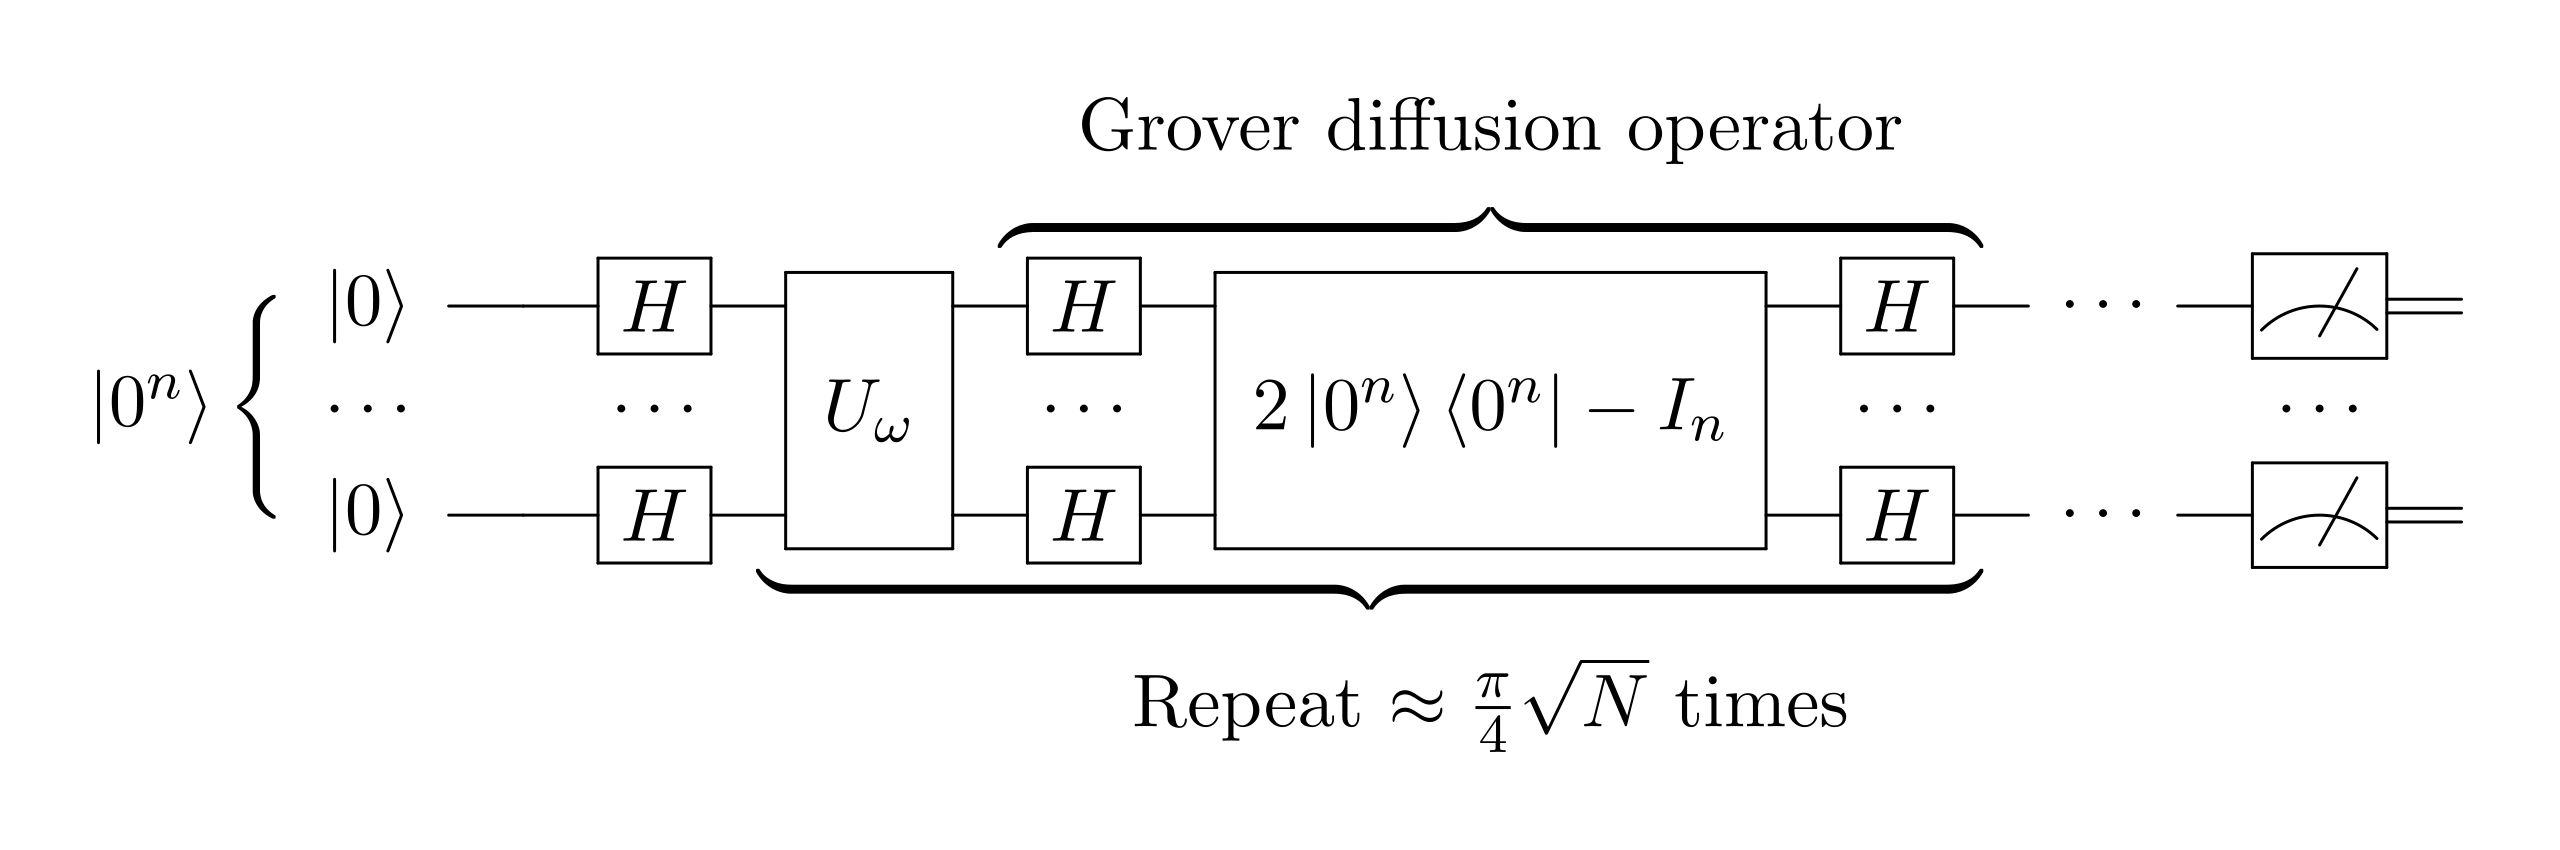
\includegraphics[width=1\textwidth]{img/grover-wiki}
  \caption{Quantum circuit for Grover search, taken from Wikipedia.}
  \label{fig: grover}
  \vspace{-30pt}
\end{figure}

\noindent This is a relatively tame example, but illustrates the basic
problem: what the circuit \emph{does} is not the same as what the
circuit \emph{is}. We cannot tell the first from the second.
We can try to rectify the problem with ``macros'', that is,
abstraction boxes which stand for more complex expressions, and that
helps. But defining a macro like the diffusion operator
\[
  D = 2 |0^n\rangle\langle 0^n| - I
\]
does not immediately help us understand what the operator is doing in
our algorithm.
A better hint comes from the oracle $U_\omega$, which is
\emph{defined} by its behaviour on basis states as
\[
  U_\omega |\kappa\rangle = (-1)^{\delta_{\omega,\kappa}} |\kappa\rangle
\]
where $\omega$ and $\kappa$ are $n$-bit (classical) strings.
This is easy to explain: it flips the phase of $|\omega\rangle$ and
leaves anything else alone.

Algebraic quantum programming takes this hint radically.
Oracles are operators with specified behaviour, so we make the whole
foundation of the approach operators with specified behaviour.
Instead of a Hilbert space $\mathcal{H}$, we focus on the operators
$\mathcal{B}(\mathcal{H})$, and in fact to avoid relying on Hilbert
space we define \emph{abstract} operator algebras
% \sidenote{In terms of Taoist cosmogony, this
%   is the One.}
$\mathcal{A}$ called
\emph{C${}^*$-algebras} which carry a linear structure, allow
multiplication $A, B \mapsto A \cdot B$, taking of adjoints $A \mapsto
A^*$, and finally have a notion of
size $A \mapsto \Vert A \Vert$.
\marginnote{
  \vspace{-30pt}
  \begin{center}
    \hspace{-10pt}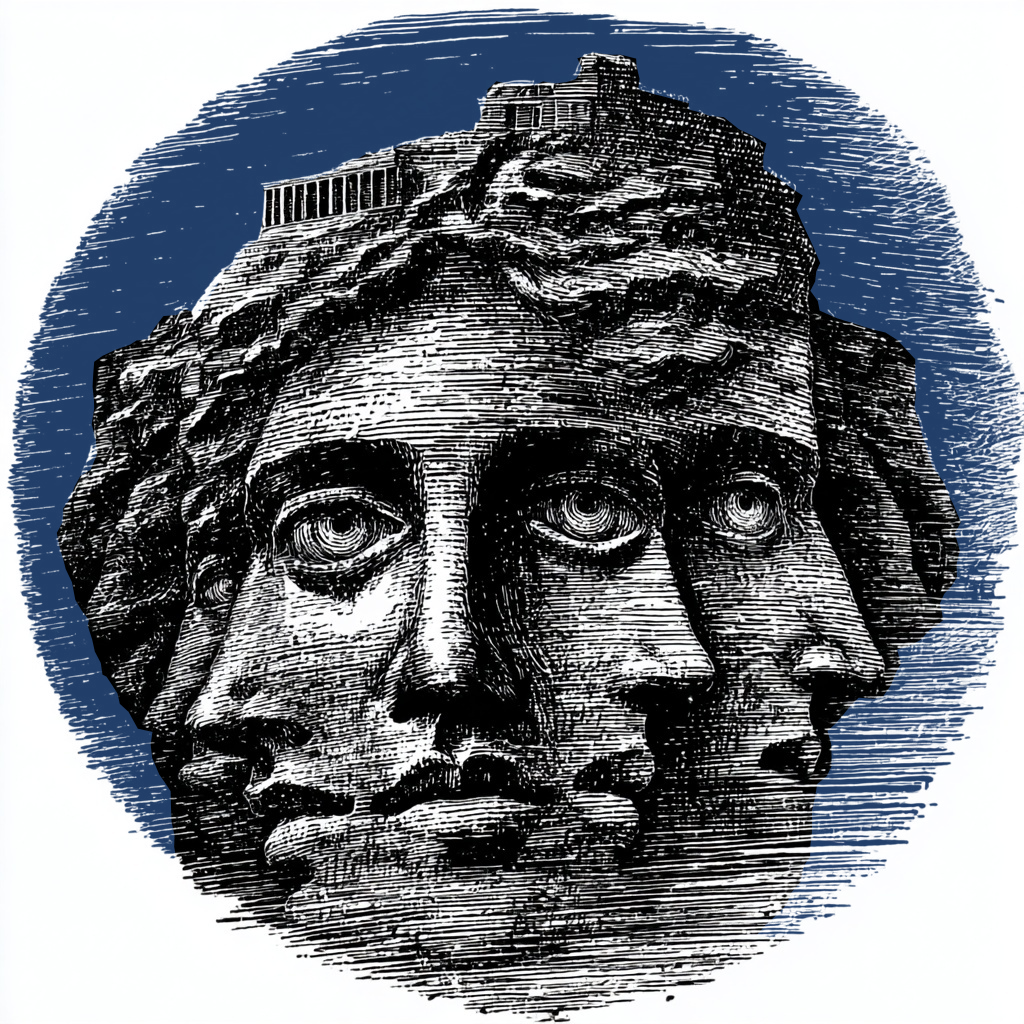
\includegraphics[width=1\linewidth]{img/oracle2}
  \end{center}  \vspace{-5pt}
  \emph{An edifice built of oracles.
    %The many oracles of quantum computing.
  } \vspace{-10pt}
} These can always be realized on a specific, concrete Hilbert
space, and indeed, this is what allows us to compile our programs on
conventional quantum computers. Although we touch on the issue of
compilation below, we leave a deeper exploration to upcoming work, and
focus instead on how to formulate algorithms when ``everything is an
oracle''.

This proceeds in a few stages. Keeping the operator algebra abstract
has the advantage that we can specify in different ways.
For instance, the algebra of a qubit $\mathcal{A}_2$ can be viewed as
the unit matrices
\[
  E_{11} =
  \begin{bmatrix}
    1 & 0 \\ 0 & 0
  \end{bmatrix}, \quad
  E_{12} =
  \begin{bmatrix}
    0 & 1 \\ 0 & 0
  \end{bmatrix}, \quad
  E_{21} =
  \begin{bmatrix}
    0 & 0 \\ 1 & 0
  \end{bmatrix}, \quad
  E_{22} =
  \begin{bmatrix}
    0 & 0 \\ 0 & 1
  \end{bmatrix}.
\]
These have a very sparse multiplicative structure:
  \begin{equation}
  E_{ab}E_{cd} = \delta_{bc}E_{ad}.\label{eq:pres-e}
\end{equation}
An alternative parameterization is given by the celebrated Pauli
matrices $\sigma_1 = X, \sigma_2 = Y, \sigma_3 = Z$, with the explicit
matrix expressions
  \begin{equation}
  \sigma_1 =
  \begin{bmatrix}
    0 & 1 \\ 1 & 0
  \end{bmatrix}, \quad
  \sigma_2 =
  \begin{bmatrix}
    0 & i \\ -i & 0
  \end{bmatrix}, \quad
    \sigma_3 =
  \begin{bmatrix}
    1 & 0 \\ 0 & -1
  \end{bmatrix}.\label{eq:pauli-mats}
\end{equation}
These have a much richer multiplicative structure:
\begin{equation}
  \sigma_i \sigma_j = \delta_{ij} I + i \epsilon_{ijk}
  \sigma_k,\label{eq:pauli-rel}
\end{equation}
where $\epsilon_{ijk} = \mbox{sgn}(ijk)$ is the Levi-Civita tensor.
These are unitary and Hermitian, so they act both as transformations
(unitary) and measurements (Hermitian), explaining their ubiquity for
quantum computing. Finally, this set of operators is ``overcomplete''
in the sense that we can generate all three from products of two, for
instance $X$ and $Z$. So a more convenient parameterization for some
purposes is simply $X$ and $Z$, which \emph{anticommute}:
\[
  XZ = -ZX.
\]
We could go on, but the point is that these all span the same set of
operators $\mathcal{B}(\mathcal{H}_2)$, but the useful computational
properties live in the multiplicative rather than the additive
structure.

To foreground and flexibly parameterize this multiplicative structure,
it helps to define the operator algebra independent of the Hilbert
space on which it acts. We do this using the method of
\emph{presentations}, where a C${}^*$-algebra $\mathcal{A} = \langle\mathcal{G}|\mathcal{R}\rangle$ is defined
in terms of the operators $\mathcal{G}$ that multiplicatively generate the full
algebra, and the relations $\mathcal{R}$ they satisfy. This replaces the explicit
matrix description, For instance, the $XZ$ parameterization corresponds to presentation
\[
  \mathcal{A}_2 = \langle X, Z | XX^* = X^2 = ZZ^* = Z^2 = I, \, XZ
  = -ZX\rangle,
\]
i.e. $X$ and $Z$ are Hermitian unitaries that anticommute.
This makes the ``oracular'' nature of programs clear.

Of course, we cannot dispense with states; they are the bridge from
abstract operators to physically realized measurements. % \sidenote{These
  % are the Two.}
But instead of
thinking of them as vectors in a Hilbert space, we view them as
probability distributions over measurement outcomes $S(\mathcal{A})$, or rather,
\emph{expectation functionals} $\mathbb{E}_\pi:
\mathcal{A}\to\mathbb{C}$ over operators.
Like the expectation functions familiar from probability theory, they
are linear in their inputs and normalized:
\[
\mathbb{E}_\pi[\alpha A + \beta B] = \alpha\mathbb{E}_\pi[A] + \beta\mathbb{E}_\pi[B], \quad  \mathbb{E}_\pi[I] = 1.
\]
Choosing an initial state like $|0^n\rangle$ corresponds here to choosing an ``eigenfunctional'' of some operator, meaning
the operator has zero variance. For instance, an
eigenfunctional $\mathbb{E}_\pi$ of $Z$ satisfies
\[
  \mathbb{E}_\pi[|Z|^2] =  \mathbb{E}_\pi[Z^2] =   \left|\mathbb{E}_\pi[Z]\right|^2.
\]
This makes sense if we view states as measurement averages; an eigenfunctional corresponds to an eigenstate,
where we always observe the same thing so the variance in outcome is
zero.

To actually enumerate different states, Hilbert space becomes
indispensable.
The \textsc{Gelfand-Naimark-Segal (GNS) Construction} allows us to
build a Hilbert space $\mathcal{H}_\pi$ directly from an operator algebra $\mathcal{A}$
and a state $\mathbb{E}_\pi$; this gives a list of ``pure states''
from which we can build expectation functionals by mixing.
Listing pure states is analogous\sidenote{In fact, it is more than
an analogy: these are both instances of a generalized Stone
duality over different fields.} to the way we can list
truth-value assignments in classical Boolean; our list is
exponentially large, but exhaustive and therefore helpful
when we need to look for (counter)examples. On the flip side, we use Boolean algebra to manipulate digital
circuits, and the C${}^*$-algebraic approach is the analogue quantum circuits.
This explains (at least at a high-concept level) why building
restricting quantum computing to Hilbert space creates problems.
It's like doing classical computing entirely with truth tables!
%the Hilbert space-first approach runs into trouble.

Once we have an algebra $\mathcal{A} = \langle
\mathcal{G}|\mathcal{R}\rangle$ and the dual perspective afforded by
states $\pi \in S(\mathcal{A})$ (including the GNS Hilbert space
$\mathcal{H}_\pi$), we almost have enough ingredients to start baking algorithms.
The only thing missing is the ability to \emph{combine} things.
There are three basic methods of composition: %\sidenote{The Three.}
\begin{itemize}[itemsep=-1pt]
\item spatial composition, aka the \emph{tensor product};
\item temporal composition, aka \emph{conjugation}; and
\item functional composition, aka \emph{quantum channels}.
\end{itemize}
The tensor product takes objects in different algebras (operators,
states, etc) and configures them simultaneously. For instance, acting with
operator $A \in \mathcal{A}$ and $B \in \mathcal{A}'$ at the same time
corresponds to the operator $A \otimes B \in \mathcal{A} \otimes
\mathcal{A}'$. Entanglement is simply the failure of an object to
tensor-factorize.
% , for instance, if $\pi_b = \mathbb{E}_b$ is the
% eigenfunctional of $Z$ with eigenvalue $b$, then
% \[
%  \Phi = \frac{1}{2}(\pi_0 \otimes \pi_0 +   \pi_1 \otimes \pi_1)
% \]
% cannot be written in the form $\Phi = \pi \otimes \rho$ for any states
% $\pi, \rho \in S(\mathcal{A}_2)$.
% % The fact that we cannot understand the behaviour entirely in terms of
% % local components (since the state does not factorize) leads to
% % ``spooky action at a distance'' as we will see below.
% This leads to a local behaviour that is not predictable from the local
% state, aka ``spooky action at a distance''.

If the tensor product captures spatial composition, \emph{conjugation}
captures composition in time.
More precisely, the Heisenberg evolution of an observable $A$ is given
by
\[
  A \mapsto U^* A U = U \triangleright A,
\]
where $U$ is the time evolution operator, and $\triangleright$ is the \emph{(operator)
  conjugator}.\sidenote{We use $\triangleright$ instead of the
  conventional $\text{Ad}_U$ action since we find the infix notation
  cleaner.}
We define the \emph{state conjugator} $\triangleleft$ as the
``pullback'' of operator conjugation:
\[
( U \triangleleft \pi) [A] = \pi( U \triangleright A) = \pi (U^*AU).
\]
This is the appropriate Schr\"{o}dinger evolution when the state is
related to vectors in a Hilbert space by $\pi(A) = \langle \pi |A
|\pi\rangle$.
Strictly speaking, we could view multiplication $A, B \mapsto A \cdot
B$ as composition in time (``do $B$, then $A$''), but time \emph{evolution} via conjugation
is a richer temporal notion than simple multiplication.

Finally, we can compose via \emph{channels}.
Channels model noisy processes and measurements.
% This is the most sophisticated way to combine elements of a program.
A channel is a generalized form of conjugation, where instead of
conjugating with one operator, we conjugate with
several. Schematically, for a family of operators $K_\lambda$ labelled by $\lambda
\in \mathfrak{L}$ that sum to the identity, $\sum_{\lambda\in
  \mathfrak{L}} K_\lambda K_\lambda^* = I$, the associated operator and state channels are the sum
of operator and state conjugators:
\[
  \mathcal{C}_{\mathfrak{L}} = \sum_{\lambda\in \mathfrak{L}}
  K_\lambda\, \triangleright, \quad   \mathcal{C}^{\mathfrak{L}} = \sum_{\lambda\in \mathfrak{L}}
  K_\lambda \,\triangleleft
\]
If the channel is \emph{observed} in state $\pi$, then outcome
$\lambda$ is measured with probability\sidenote{The requirement that
  $K_\lambda K_\lambda^*$ sums to unity then corresponds to
  conservation of probability.} $p_\lambda$ given by the \textsc{Born
  rule} as
\[
  p_\lambda = \pi[K_\lambda K_\lambda^*],
\]
and the channel (conditioned on this outcome) according to the
\textsc{L\"{u}ders rule} by
\[
  \mathcal{C}_{\mathfrak{L}} \mapsto p_\lambda^{-1} K_\lambda\,
  \triangleright, \quad \mathcal{C}^{\mathfrak{L}} \mapsto
  p_\lambda^{-1} K_\lambda \,\triangleleft.
\]
The canonical example is \emph{projector-valued measurement (PVM)},
where the $K_\lambda$ are orthogonal projectors that resolve the identity:
\[
  \sum_{\lambda} \Pi_\lambda = I, \quad \Pi_\lambda \Pi_\mu = \delta_{\mu\lambda}\Pi_\lambda.
\]
In state $\pi$, we observe outcome $\lambda$ with probability
$p_\lambda = \pi(\Pi_\lambda)$, and the post-measurement state is
$p_\lambda^{-1}\Pi_\lambda \triangleleft \pi$.\sidenote{This rule may be familiar from a first course on quantum
computing. See for instance the drily canonical reference
  \emph{Quantum Computation and Quantum Information} (2000), Nielsen
  and Chuang.}

From these primitives, we can build everything else.
% \marginnote{
%   \vspace{-0pt}
%   \begin{center}
%     \hspace{-10pt}\includegraphics[width=1\linewidth]{img/goldberg}
%   \end{center}  \vspace{-5pt}
%   \emph{Composition begets $\sim 10^4$ Things.
%   } \vspace{5pt}
% }
% \sidenote{The Ten
%   Thousand things. We won't belabour the analogy any further.}
As a simple example of how this works, we can start by defining the
\emph{generalized Clifford} or simply \emph{qudit algebra}\sidenote{Known by many other names, including the generalized Pauli, Weyl-Heisenberg, or Sylvester matrices.}
\begin{equation}
  \mathcal{A}_d = \langle X, Z | XX^* = X^d = ZZ^* = Z^d = I, \, ZX =
 \omega_d XZ\rangle,\label{eq:pres-qudit}
\end{equation}
where $X$ and $Z$ are \emph{unipotent} unitaries whose $d$th power is
the identity, and \emph{braid}, i.e. commute
up to a $d$th root of unity $\omega_d = e^{2\pi i /d}$.
We can factorize the unipotence relation of $Z$ to obtain its eigenvalues,
\[
  Z^d - I = \prod_{k=0}^{d-1} (Z - \omega_d^k I),
\]
and build the projector onto $\omega_d^k$ explicitly as
\[
  \Pi_{k}^{(Z)} = \frac{\prod_{j\neq k}(Z - \omega_d^j
    I)}{\prod_{j\neq k}(\omega_d^k - \omega_d^j)}.
\]
Using projectors and working on the tensor product
$\mathcal{A}_d^{\otimes 2}$, we can define a controlled-$X$ operation:
\[
  \text{CX} = \sum_{k=0}^{d-1} \Pi_{k}^{(Z)} \otimes X^k,
\]
which applies $X^k$ in the second slot when it encounters $\pi^{(Z)}_k$, the
$\omega_d^k$-eigenfunctional of $Z$, in the first.
You can show that $X \triangleleft \pi^{(Z)}_k =
\pi^{(Z)}_{k+1}$,\footnote{This is easy to derive from the braiding
  relation: \[
    ZX |\omega_d^k\rangle = \omega_d X Z |\omega_d^k\rangle =
    \omega_d^{k+1} X |\omega_d^k\rangle.
  \]} and it follows that
\[
  \text{C}X (X^k \otimes I) \triangleleft (\pi^{(Z)}_0 \otimes
  \pi^{(Z)}_0) = (X^k \otimes X^k) \triangleleft (\pi^{(Z)}_0 \otimes
  \pi^{(Z)}_0).
\]
Extending to a sum of terms $W = \frac{1}{\sqrt{d}}\sum_{k=0}^{d-1}
X^k$, we have\sidenote{This is a special form of the \emph{quantum Fourier
  transform (QFT)} that we cover at greater depth below. More
generally it takes the form $W = \frac{1}{\sqrt{d}}\sum_{k=0}^{d-1}
X^kZ^{-(k+1)}$.}
\[
    \text{C}X \left(W\otimes I\right) \triangleleft (\pi^{(Z)}_0 \otimes
  \pi^{(Z)}_0) = \frac{1}{\sqrt{d}}\sum_{k=0}^{d-1}\left(X^k \otimes X^k\right) \triangleleft (\pi^{(Z)}_0 \otimes
  \pi^{(Z)}_0),
\]
or in the GNS Hilbert space associated with $\pi^{(Z)}_0$,
\[
  \text{C}X (W\otimes I)|0\rangle\otimes 0\rangle =
  \frac{1}{\sqrt{d}}\sum_{k=0}^{d-1} |k\rangle\otimes k\rangle.
\]
This state has the miraculous property that the outcome of a $Z$
measurement on the first system\sidenote{This is the PVM with components $\Pi_k^{(Z)} \otimes I$ for
$k \in \{0, 1, \ldots, d-1\}$; similarly, a $Z$ measurement on the second system
has projectors $I\otimes\Pi_k^{(Z)} $.} automatically matches the outcome of a
$Z$ measurement on the second; this is ``spooky action at a distance''.
We have just performed our first nontrivial quantum algorithm, and
produced an entangled state.
% We can choose the first state to be\sidenote{This is $\pi^{(X)}_0$ because the sum is invariant
%   under multiplication by $X$.}
% \[
% \pi^{(X)}_0 = \frac{1}{\sqrt{d}}\big(I + X + X^2 + \cdots + X^{d-1}\big)
% \triangleleft \pi^{(Z)}_0,
% \]
% and the second to be plain old $\pi^{(Z)}_0$. Then, since  $X
% \triangleleft \pi^{(Z)}_k = \pi^{(Z)}_{k+1}$, it follows that
% \[
%   \frac{1}{\sqrt{d}} \sum_{k=0}^{d-1} |k\rangle |k\rangle =
%   \frac{1}{\sqrt{d}} \sum_{k=0}^{d-1} (X^k \otimes X^k) |0\rangle |0\rangle.
% \]
% when we take the GNS ``slice'' 

% Although $Z$ is no longer Hermitian, it is diagonalizable, with
% eigenvalues $\omega_3^\ell$ for $\ell = 0, 1, 2$, so we can single out
% the $\ell = 0$ eigenfunctional $\pi$, satisfying
% \[
%   \text{var}_\pi(Z) = \mathbb{E}_\pi[|Z|^2] -
%   \left|\mathbb{E}_\pi[Z]\right|^2 = 0, \quad \mathbb{E}_\pi[Z] = 1.
% \]
% We can use the GNS construction to create a Hilbert space
% $\mathcal{H}_\pi \cong \mathbb{C}^3$
% % In this paper, we
% % will see how to construct teleportation, Grover search, Shor's algorithm,
% % Hamiltonian simulation, and basic quantum error correction, leaving
% % more advanced applications for elsewhere.

This little construction already contains the whole ethos of the paper.
%Nothing here depended on drawing a circuit, choosing a basis, or
%committing to a particular hardware model.
We specified an algebra
by generators and relations, treated states as expectation functionals,
and then \emph{composed} until something recognizably algorithmic
fell out.
%This construction illustrates the algebraic workflow in miniature.
In what follows, we apply the same philosophy to five canonical
protocols---teleportation, Grover search, Fourier sampling, simulation, and
error correction---which not only demonstrate different aspects of algebraic
quantum programming, but in turn, are illuminated by the algebraic
perspective.
We may draw fewer circuits, and fall out of touch with
compilation-level details, but we trade ``how'' for ``why'', with
intuition and unifying themes emerging elegantly from the algebra. It's
a good trade.
% When operators come first, it is often clearer \emph{why}
% something works, at the corresponding expense of \emph{how} it works.
% \sidenote{A
% similar tradeoff occurs in classical programming languages, where
% high-level abstraction can obscure low-level implentation.}
% But while ``how'' is important, it can obscure the common mechanisms
% at play;
% We will trade a little ``how'' for a little ``why'', moving away from
% gate-level compilation but seeing common themes emerge, with
% mathematical elegance
% and computational necessity, from the algebra. It's a good trade.
% In that sense, yaw is not ``a new gate set'' but a way of
% keeping the multiplicative structure in the foreground: the relations
% \emph{are} the program.
% The rest of the paper takes five canonical protocols and uses each as a
% controlled experiment: if we rebuild the familiar story using only
% presentations, states, and the three composition laws, what does the
% algebraic viewpoint bring into view?
% make unusually explicit?